\documentclass[journal]{IEEEtran}
\usepackage{amsmath,amssymb,booktabs,array,tabularx,graphicx,cite,xurl}
\usepackage[hidelinks]{hyperref}
\hypersetup{pdftitle={Supplementary Evidence and Reproduction Records: Hierarchical RF Tokenization},pdfauthor={Anonymous working draft}}
\graphicspath{{figures/}}
\setlength{\tabcolsep}{4pt}
\begin{document}
\title{Supplementary Evidence for Hierarchical RF Tokenization}
\InputIfFileExists{author_metadata.tex}{}{\author{Anonymous working draft}}
\maketitle
\setcounter{figure}{8}
\setcounter{table}{8}

\section{LoRa Cohorts and Baseline Reproduction}
\subsection{Common Packet and Receiver Protocol}
For each transmitter--receiver cell, packet selection uses seed 20261012. The first 160 of 200 fixed selected rows train the source classifiers and the remaining 40 support validation. At a held receiver, all 200 selected rows per transmitter are evaluated. Each of two receiver folds uses seeds 201, 202, and 203. HStem, Shen, FAN, and IB used CPU FP32 in the archived external reporting pass. ASKNet and Spec+Siamese used CUDA FP32. The separately matched tokenizer pass used common GPU inference for all three arms (FP32, matmul TF32 off, cuDNN TF32 on, batch 128). HStem scores 97.333\% in Native and 97.335\% in the matched tokenizer pass. The bootstrap seeds are 24016 for the original external comparisons and 26026 for the same-support comparison.

Table~\ref{tab:protocol-context} records the original LoRa contexts. The Triad-GAN numbers summarize vector bar heights after removing the source receivers in each training condition \cite{wang2026triad}. The heterogeneous mean uses 15 receivers, omitting RTL-1, Pluto-1, B200-1, B200-mini-1, and B210-1. The corresponding homogeneous mean is approximately 84.4\%. RIFLE reports a cross-receiver mean for partial TX--RX coverage \cite{zhang2026rifle}. The companion CIS and RA results use its 14-to-6 receiver split \cite{oobcompanion}. The main-paper accuracy comparison uses a common packet protocol and cohort.

\begin{table*}[!t]\centering
\caption{Published and historical LoRa protocol context. Each score is tied to its own data availability and exposure.}
\label{tab:protocol-context}% Published protocols and the two project results are explicitly identified.
\begin{tabularx}{\textwidth}{@{}ll>{\raggedright\arraybackslash}Xl@{}}
\toprule
Study / method & Source and evaluation RXs & Training data or evaluation condition & Accuracy (\%)\\
\midrule
Shen et al.\ \cite{shen2024receiver} & 5 heterogeneous / 20 tested & 800 captures per source TX/RX before augmentation & Per RX (Fig.~9b)\\
Ma Spec+Siamese \cite{ma2025robust} & 2 source / 20 tested & 800 source packets per TX/RX; high-SNR test dataset A & Per RX (Fig.~11)\\
Triad-GAN \cite{wang2026triad} & 5 heterogeneous / 15 held out & Equal mean over held-out bars digitized from Fig.~5(b) & $\approx95.8$\\
RIFLE \cite{zhang2026rifle} & 20-RX corpus & Partial TX--RX coverage; published cross-RX mean & 93.90\\
ASKNet \cite{liu2026ask} & N210-1 / RTL-6 & 5,600 training packets in rerun; Day 2--4 mean & 84.52 (log) / 95.48 (rerun)\\
Companion CIS / RA \cite{oobcompanion} & 14 source / 6 held out & Historical companion experiments & 99.24 / 99.14\\
HStem (this work) & 5 source / 5 held out per fold & 160 training packets per TX/RX; two folds, three seeds & 97.333\\
\bottomrule
\end{tabularx}

\end{table*}

\subsection{Primary Baseline Implementations}
\textit{Shen CE and DANN.} The two arms share the same $52\times126$ CIS input and residual encoder/TX head. The TensorFlow-to-PyTorch implementation passed 103 forward and gradient parity checks. The adaptation corrects a misaligned RX validation-label slice in the author entrypoint and fixes validation noise across epochs. The arms share initial encoder and TX weights and noise streams, and use batch 64, SGD at $10^{-3}$, .9 momentum, a 500-epoch cap, and plateau and early-stop rules. DANN adds the source-RX gradient-reversal objective. DANN minus CE is \(+0.673\) pp Native with conditional interval \([0.208,1.233]\), and \(-0.070\) pp Strict-IB with interval \([-0.247,0.152]\) \cite{shen2024receiver}.

\textit{Ma Spec+Siamese.} Our paper-derived from-scratch arm uses a shared nine-convolution residual extractor, pooling, 512- and 256-unit layers, and a TX head \cite{ma2025robust}. Each epoch visits every source training example as an anchor and samples a same-TX, different-source-RX partner. Thirty-two pairs make a batch of 64 views with independent channel and noise draws. The objective adds example means of TX cross-entropy and NT-Xent with temperature .05. The log-magnitude STFT uses 128 rectangular samples, hop 64 and a centered 52-bin crop, giving \(52\times127\). SAME padding and \(2\times2\) average pooling yield a \(13\times32\times64\) feature map. The exponential five-tap channel model uses fractional delays and an eight-tone low-Doppler Jakes approximation, with 5--300 ns delay, 0--5 Hz Doppler and 10--40 dB SNR ranges.

Adam starts at \(3\times10^{-4}\), halves after ten epochs of stalled source-validation CE, and stops after 30 unimproved epochs or 160 total epochs. Training uses BF16 GPU autocast for network operations and FP32 processing for features and losses. Source validation and report inference use FP32. Source accuracy ranges from 99.05\% to 99.45\%; one fit stops at epoch 156 and five reach 160. The six fits contribute 239,000 updates and 60,000 held packet predictions. The published pretraining variant uses additional data; P-H5\(\times\)160 evaluates the from-scratch variant.

\subsection{Additional Adaptations}
Table~\ref{tab:adaptations} retains the complete Native and available Strict-IB summaries. \textit{FAN and IB-RFF} use the released frequency-aware backbone adapted to length 8192, with patch 512, stride 256 and 31 tokens of width 128. FAN and the second-stage IB-RFF use Adam at \(10^{-3}\), batch 128, a 200-epoch cap, and source-validation early stopping. IB starts from the matching FAN checkpoint and uses CPU normalized-HSIC with the previously fixed .004 coefficient. Stage 2 minus stage 1 is \(+0.978\) pp in Native and \(+3.983\) pp in Strict-IB with conditional intervals \([-0.037,2.195]\) and \([3.373,4.582]\). The \href{https://github.com/BeechburgPieStar/IB-RFF/tree/5a03a04da86c4bbf5cf90f41a55c268bf2152203}{public IB-RFF release} supplies WiSig code, logs and weights. The exact recipe and checkpoint for the published LoRa receiver-and-day result are unavailable in that release \cite{wang2026ib}.

\begin{table*}[!t]\centering
\caption{Additional P-H5\(\times\)160 adaptations. Accuracies, F1 and worst-RX means are percentages. The \(\pm\) terms are sample fit SDs in pp.}
\label{tab:adaptations}% Generated from the submission evidence ledger.
\begin{tabular}{lrrrrrr}
\toprule Method & Native Acc. & Strict-IB Acc. & Native F1 & Strict F1 & Native Worst & Strict Worst\\
\midrule
FAN & 72.555 $\pm$ 2.683 & 75.827 $\pm$ 2.351 & 71.309 & 75.136 & 62.250 & 71.783\\
IB-RFF & 73.533 $\pm$ 2.873 & 79.810 $\pm$ 2.731 & 72.427 & 79.291 & 63.450 & 75.683\\
ASKNet & 65.092 $\pm$ 31.936 & Deferred & 62.995 & -- & 58.900 & --\\
Gul Federated & 42.725 $\pm$ 3.798 & -- & 37.311 & -- & 33.883 & --\\
\bottomrule
\end{tabular}

\end{table*}

\textit{ASKNet.} The six P-H5\(\times\)160 fits use the public default candidate set, 8191 complex transformation modes, batch 128, Adam at \(10^{-3}\), a 200-epoch cap and patience 20 \cite{liu2026ask}. Held accuracies in fold--seed order are 87.220/40.670/74.520/87.130/89.320/11.690\%. Corresponding source accuracies are 90.650/40.050/77.350/90.550/91.250/11.500\%. The last fit selects epoch 1 and stops at epoch 21. Weak fit and validation results contribute to the reported dispersion. The \href{https://github.com/BeechburgPieStar/ASKNet-RFF/blob/f00846d68425315b68ae69b8c6b712e08559c2fe/Lora/logs/h5_rescisnet_k10_per800_trainrxn210_1_day1_seed2023.k_trace.txt}{author log} uses eight cutoff candidates and 4095 modes on a separate public receiver-drift protocol. The locked, single-seed rerun on that protocol selected by source CE and obtained 95.48\% on RTL-6 Days 2--4, compared with the author log's 84.52\%. The learned cutoffs were 768 and 512, respectively. The \href{https://github.com/hanCChan/crossatten/blob/59c44e1/research/s44_baseline_verification/RESULTS.zh-CN.md}{verification record} gives dataset identifiers, environment, configuration and correct counts.

\textit{Gul Federated.} Our adaptation treats each source receiver as a client in the balanced all-client training configuration \cite{gul2026federated}. A $52\times126$ CIS passes through residual widths 32/32/64/64 and a normalized 512-dimensional embedding to a TX head and a gradient-reversed RX head. Settings include source AWGN at 0--49 dB, local SGD with five epochs per round, batch 64, learning rate \(10^{-3}\), and gradient reversal \(\lambda=.01\). The server averages client weights by packet count over 200 rounds; each fit has 125,000 local updates. Training uses FP32 weights and BF16 network operations. The minimum clean source RX-equal CE selects rounds 199/200/200/199/200/198, with source accuracy 34.600--44.250\%. The authors' five-client setting uses 720 segments per TX/RX for training and reports peak evaluation accuracy, compared with 160 and source-only selection here. A single source-only diagnostic with reset local momentum .9 increased round-24 source accuracy from 13.35\% to 44.55\%. The \href{https://github.com/hanCChan/crossatten/tree/2fe246263f75/research/s43_gul_federated}{frozen comparison} retains the six trajectories and receiver-paired estimates.

\begin{table}[!t]\centering
\caption{Gul adaptation contrasts on Native, in pp. Intervals are conditional on receivers and fits.}
\label{tab:paired-gul}% Generated from the submission evidence ledger.
\begin{tabular}{lrr}
\toprule Contrast & Mean (pp) & 95\% interval (pp)\\
\midrule
HStem -- Gul Federated & $+54.608$ & $[+51.278, +58.128]$\\
Gul Federated -- Spec+Siamese & $-53.165$ & $[-57.717, -48.978]$\\
Gul Federated -- Shen-DANN & $-51.483$ & $[-56.790, -46.558]$\\
\bottomrule
\end{tabular}

\end{table}

\section{Tokenizer Controls and Feature Diagnostics}
\subsection{Pairing and Factorial Results}
The data-free parameter-matching rule selected Patch-Lite, with 134,266 parameters (0.43\% over HStem). The archived full Patch has 571,434. Long-Patch's six source-selected epochs are 156/171/171/129/159/153 from the 200-epoch schedule. In the same order the source accuracies are 95.250/96.550/96.700/96.100/96.900/96.650\%, and the held accuracies are 91.070/95.330/95.780/94.280/96.120/94.420\%. The \href{https://github.com/hanCChan/crossatten/tree/ad5443e/26-long-patch-control}{paired experiment record} contains the configurations, fit timing, raw-row provenance, joint inference records, and archived predictions' identifiers. Restore procedures retain epoch and RNG state.

\begin{table}[!t]\centering
\caption{Four BN--GELU configurations. Accuracies and macro-F1 are held-RX-equal percentages.}
\label{tab:factorial}% Generated from the submission evidence ledger.
\begin{tabular}{ccrr}
\toprule BN & GELU & Acc. & Macro-F1\\
\midrule
Yes & Yes & 97.335 & 97.326\\
Yes & No & 96.583 & 96.554\\
No & Yes & 96.145 & 96.135\\
No & No & 96.743 & 96.728\\
\bottomrule
\end{tabular}

\end{table}

The three intermediate BNs account for 352 affine parameters. The factorial shares the nominal support, fitting budget and the rest of the network (Table~\ref{tab:factorial}). Adding GELU gives \(+0.752\) pp (\([0.197,1.432]\)) with BN and \(-0.598\) pp (\([-1.150,0.168]\)) without BN. The paired interaction is \(+1.350\) pp (\([0.930,1.750]\)). Removing both intermediate operations retains 96.743\% held accuracy, compared with Long-Patch's 94.500\%. In a separate two-receiver, held-source pilot, HStem improves held accuracy by 4.583 and 1.383 pp. Its source-to-held gap shrinks by 2.437 and 0.342 pp, with the second receiver below the 0.5 pp pilot criterion.

\subsection{Effective Kernels and Source Geometry}
The round-trip kernel transform has rank 256. Its coefficients can be materialized as a standard inference convolution. Six S1 checkpoints had bit-identical logits on 12,000 source predictions after materialization. BN folding also agrees at a fixed \(10^{-4}\) logit tolerance in all six arms when TF32 is off (maximum \(5.39\times10^{-5}\)). TF32-enabled execution exceeds that tolerance (maximum approximately .01957), with classification agreement. These execution checks use the registered inputs and frozen models.

\begin{table}[!t]\centering
\caption{Source-validation final geometry. Each statistic is averaged across six fits.}
\label{tab:source-geometry}% Generated from the submission evidence ledger.
\begin{tabular}{lrrrrr}
\toprule Arm & Source Acc. & $B_{\rm TX}$ & $D_{\rm RX|TX}$ & $J_c$ & $J_w$\\
\midrule
P0 & 95.917 & 0.785 & 0.0286 & 27.585 & 4.270\\
S1 & 96.625 & 0.778 & 0.0281 & 27.818 & 4.435\\
H1 & 97.467 & 0.805 & 0.0262 & 31.225 & 4.925\\
H0 & 98.175 & 0.817 & 0.0235 & 35.577 & 5.449\\
\bottomrule
\end{tabular}

\end{table}

The effective-kernel energy at 0.25--0.5 cycles per front-end position is 21.808/7.692/4.043\% for P0/S1/H1. In the frozen 18-model join, Spearman correlations with final \(J_w\) and conditional RX scatter are \(-.556\) and \(+.410\). Figure~\ref{fig:kernels} visualizes the frozen measurements. These descriptive associations combine kernels from different interventions and operate in feature coordinates. Table~\ref{tab:source-geometry} adds total between-TX scatter and source accuracy. Centering archived SNR and CFO metadata within TX-by-RX cells yields small SNR--margin and absolute-CFO--margin rank correlations, approximately \([-.028,.058]\) and \([-.057,.032]\) across 24 models. This clarifies why marginal metadata associations cannot identify a single physical cause for held-RX errors. The \href{https://github.com/hanCChan/crossatten/tree/308bb6f/25-tifs-integration}{source geometry analyses} provide layerwise and per-fit statistics.

\begin{figure*}[!t]\centering
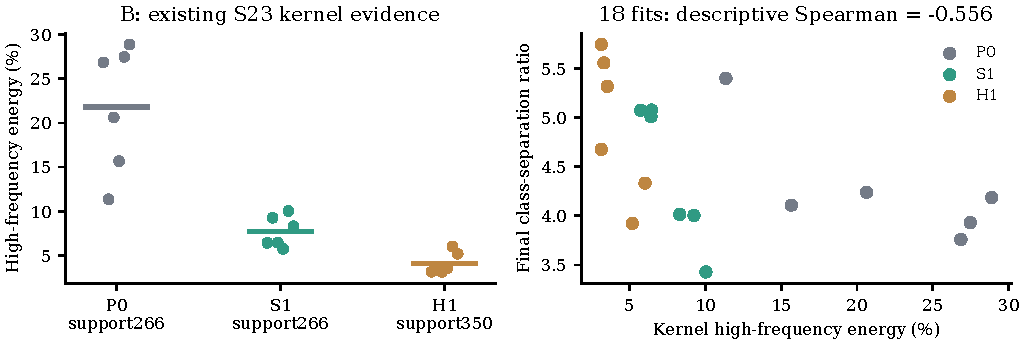
\includegraphics[width=.94\textwidth]{fig04_mechanism_B.pdf}
\caption{Frozen effective-kernel energy and the descriptive relationship to final $J_w$. The spectral bins refer to the shared front-end coordinates.}
\label{fig:kernels}
\end{figure*}

\subsection{Receiver and Synchronization Diagnostics}
HStem's Native mean exceeds Ma's on seven RTL receivers. Ma leads on B200-mini-1, Pluto-1, and B210-1. The archived HStem--DANN Native contrast is negative at B200-mini-1 and B210-1 by 2.017 and 1.217 pp and close to zero on RTL-6. Pluto-1 contributes about 82\% of the 2.632\,pp HStem--Shen-CE Strict-IB difference. The other nine receivers average 0.531 pp. Under Strict-IB, Shen-CE's Pluto-1 recalls on TX32/34/35/39 are 53.833/34.500/10.833/24.333\%, versus 94.500/79.167/82.500/88.333\% for HStem. Largest Shen-CE confusions include TX35-to-32, TX39-to-38, TX34-to-33 and TX32-to-31.

The source circular-shift test reduces HStem from 98.175\% to 21.858/17.775\% at shifts \(-4/+4\). Patch-Lite falls to 22.567/16.983\%. The shift sensitivity remains when the original FFT magnitude is held fixed. Figure~\ref{fig:limits} retains the archived shift curve and the full set of Pluto-1 TXs. These are separate diagnostic cohorts.

\begin{figure*}[!t]\centering
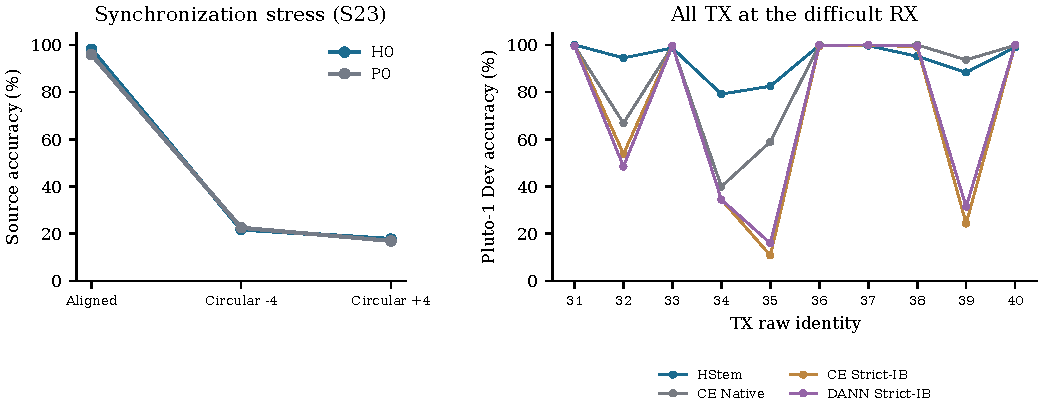
\includegraphics[width=\textwidth]{fig07_limits.pdf}
\caption{Circular-shift sensitivity on source-validation windows (left) and per-TX Pluto-1 accuracy in the archived external evaluation (right).}
\label{fig:limits}
\end{figure*}

\section{Cost and Cross-Waveform Evaluation}
The shared Native timing session uses a GeForce RTX 4060 Laptop GPU, PyTorch 2.5.0 and CUDA 12.4. Identical synthetic IQ is resident on the GPU. It times IQ-to-TX-logits under FP32 networks with AMP and TF32 disabled; Shen's CIS retains its FP64 frontend. Each model and batch size has 12 warmups and 72 measured forwards. Each of the 24 model orders is used in three blocks. The live CUDA peak includes deployed PyTorch weights, buffers, input and temporary tensors. The stored Shen-DANN and Gul checkpoints also include their training-only RX heads. The \href{https://github.com/hanCChan/crossatten/tree/2fe246263f75/research/s43_gul_federated/evidence}{same-session timing record} gives all four models and raw synchronized samples, including Gul's B1 median of 1.187 ms and B128 rate of 3,823 packets/s.

\begin{table}[!t]\centering
\caption{Separate matched tokenizer timing. Batch latencies are p50/p95 in ms.}
\label{tab:structure-timing}
\setlength{\tabcolsep}{2.5pt}
% Generated from the submission evidence ledger.
\begin{tabular}{lrrrr}
\toprule Method & Parameters & B1 (ms) & B128 (ms) & B128 packets/s\\
\midrule
Patch-Lite & 134,266 & 2.418 / 3.582 & 14.570 / 16.196 & 8,785\\
Long-Patch & 138,346 & 2.466 / 7.274 & 17.845 / 20.053 & 7,173\\
HStem & 133,690 & 2.967 / 6.047 & 17.991 / 20.709 & 7,115\\
\bottomrule
\end{tabular}

\end{table}

The matched tokenizer timing session uses the same type of GPU, three warmups and 15 samples, with matmul TF32 off and cuDNN TF32 on (Table~\ref{tab:structure-timing}). The partial operation counts are 95.028M, 55.346M, and 55.477M MACs for HStem, Patch-Lite, and Long-Patch and omit operations such as FFT. Other timing sessions, including the historical Strict-IB timings and the larger literal LoRa ASKNet, remain in the \href{https://github.com/hanCChan/crossatten/tree/bd671cd/publication/tifs_hstem/tables}{archived timing tables}. The literal ASKNet variant has 74,153,872 complex/real elements, or 141,246,353 real degrees of freedom.

The WiSig ManyRx comparison uses days 1 and 2, with 11,468 and 11,500 evaluation packets across two inner source-domain views and six held receivers per view \cite{hanna2022wisig}. The paired bootstrap resamples receivers within view. Natural accuracies are 84.46\% and 83.60\% for HStem and Long-Patch. The \(\pm10\) kHz losses are 22.61 and 27.66 pp, and equal-content \(\pm9\)-sample placement losses are 0.77 and 4.28 pp. For the CFO contrast one of four fit differences is negative; the placement contrast favors HStem in all four. The \href{https://github.com/hanCChan/crossatten/tree/b170624/research/s29_wisig}{WiSig experiment record} documents input IDs, the equal-content control and the frozen evaluation protocol.

\IEEEtriggeratref{5}
\bibliographystyle{IEEEtran}
\bibliography{references}

\clearpage
\onecolumn
\section{Frozen Source-Validation PCA Cohorts}
Each model has its own top-two PCA basis, fit to final per-packet L2-normalized embeddings. Every panel shows the 50 TX-by-RX cell centroids; color identifies TX and marker shape identifies source RX. Axes describe separate model-specific coordinate systems. The original-dimensional results are in the main manuscript and Table~\ref{tab:source-geometry}.

\begin{figure}[!ht]\centering
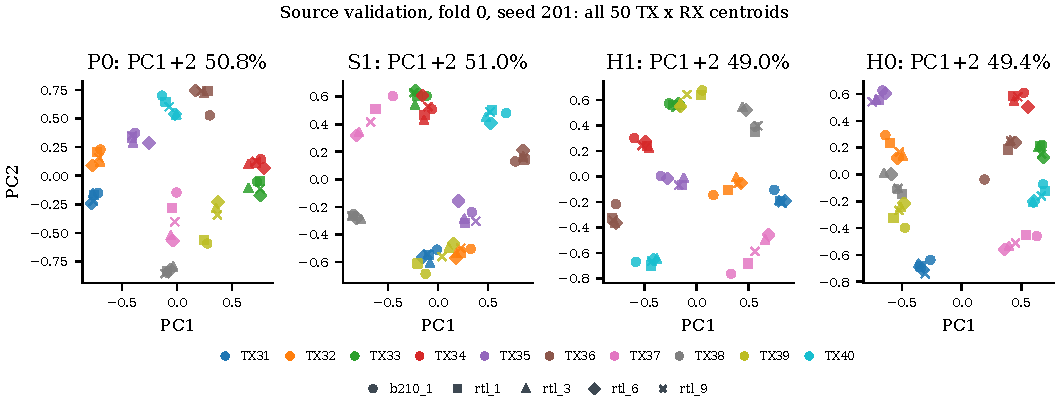
\includegraphics[width=.94\textwidth]{supp_pca_f0_s201.pdf}\par
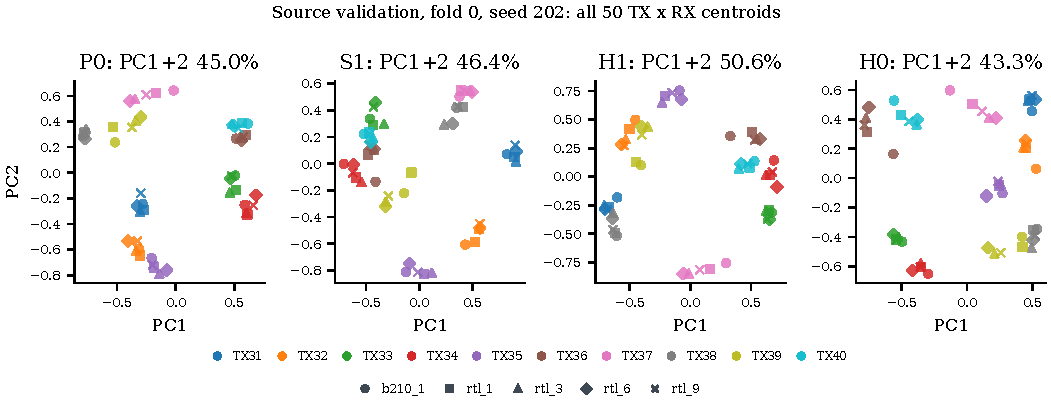
\includegraphics[width=.94\textwidth]{supp_pca_f0_s202.pdf}\par
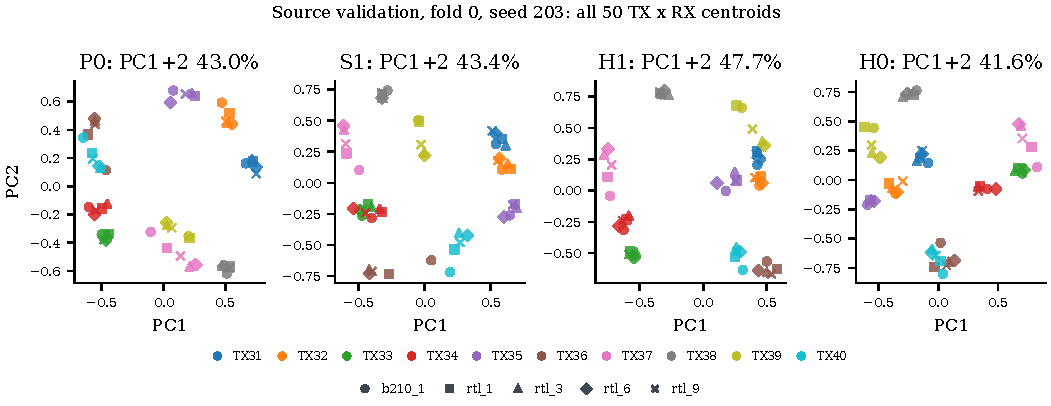
\includegraphics[width=.94\textwidth]{supp_pca_f0_s203.pdf}
\caption{All three fold-0 seeds in ascending order. Each row shows Patch-Lite, S1, H1, and HStem.}
\end{figure}
\clearpage
\begin{figure}[!ht]\centering
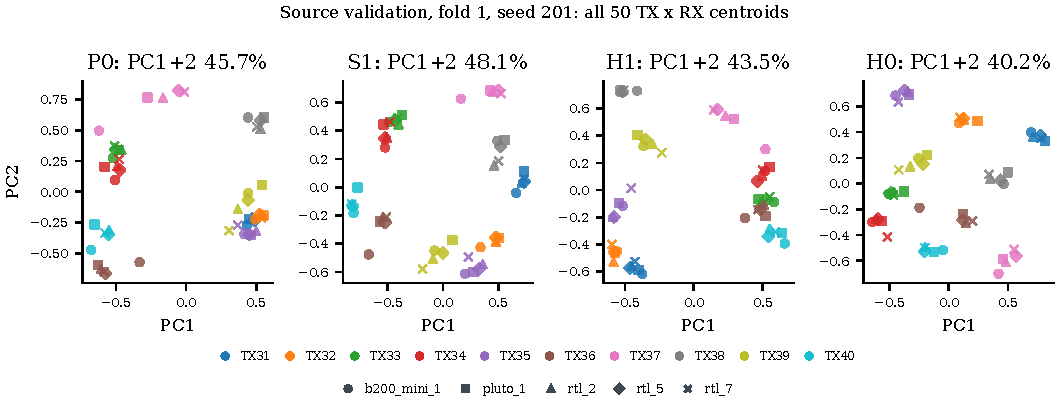
\includegraphics[width=.94\textwidth]{supp_pca_f1_s201.pdf}\par
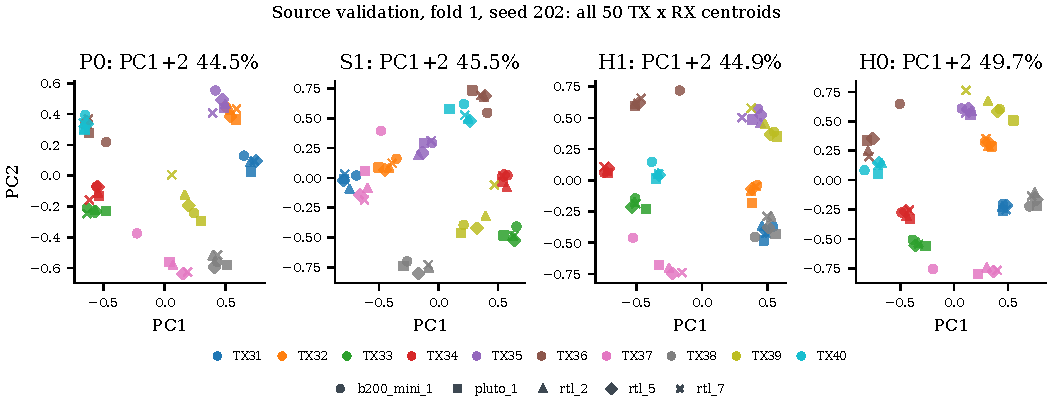
\includegraphics[width=.94\textwidth]{supp_pca_f1_s202.pdf}\par
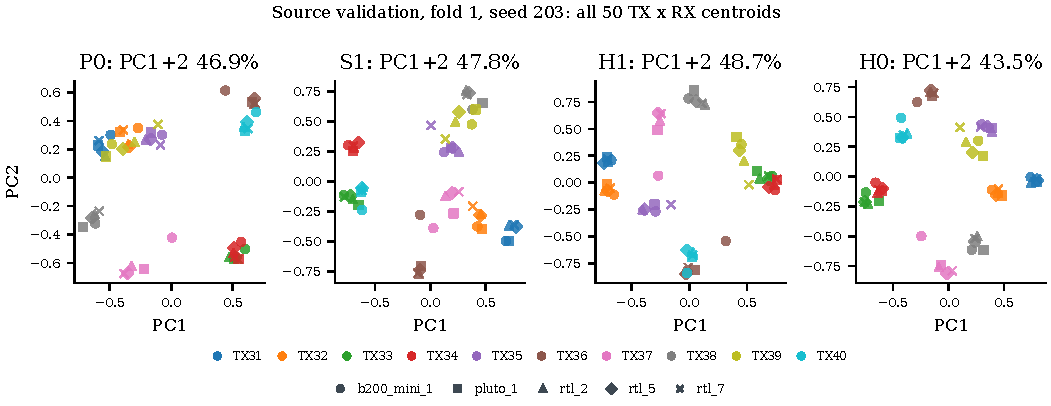
\includegraphics[width=.94\textwidth]{supp_pca_f1_s203.pdf}
\caption{All three fold-1 seeds in ascending order. Each row shows Patch-Lite, S1, H1, and HStem.}
\end{figure}
\end{document}
